%\chapter{Designing, Building, and Testing a \texorpdfstring{Nb$_3$Sn}{Nb3Sn} Axion cavity Using Nb and Evaporated Cu-Sn}\label{sec:CavityRF}

\chapter{Superconducting RF Results}\label{sec:CavityRF}

In this dissertation, the critical temperature and the width of the magnetic transition to the superconducting state have been used to assess the quality of Nb$_3$Sn films and to infer information about composition homogeneity and strain state. However, magnetometry techniques do not provide information about RF behavior, making quality factor measurements in a resonator setup a more conclusive evaluation of superconducting films for RF cavity applications. Quality factor measurements in a magnetic field are especially useful for providing feedback to film synthesis that is directly relevant to axion detector applications, whether that field is entirely composed of the AC RF magnetic field or a combination of a large background DC field and a small resonator AC field.


Two strategies were used to measure the RF properties of superconducting samples:
\begin{enumerate}
    \item \textbf{Small-sample method}: Place a small superconducting sample in a large resonant cavity of known material, and extract the quality factor of the superconducting sample
    \item \textbf{Full-coating method}: Coat the entire resonating surface with the superconducting material, and measure the total quality factor
\end{enumerate}

\noindent For the small-sample method (1), the measured $Q$ depends on both the sample and the host cavity through a weighted average:

\begin{equation}
    R_{s,\text{total}} = \frac{\sum_i A_i R_{s,i}}{\sum_i A_i}
\end{equation}

\noindent where $A_i$ is the surface area and $R_{s,i}$ is the surface resistance of region $i$. The measured quality factor is then $Q_\text{measured} = G/R_{s,\text{total}}$, where $G$ is the geometric factor. If the host cavity has an area $A_\text{host} \gg A_\text{sample}$ and $R_{s,\text{host}} \gg R_{s,\text{sample}}$, the host resistance dominates the measurement regardless of the sample's superior properties. This error can be reduced by using a high-$Q$ superconducting host cavity where the sample's contribution is more significant.

In both methods, antenna coupling losses can be accounted for (Sec.~\ref{sec:Qantenna}). However, the full-coating method (2) requires separate calculation of RF leakage at seams (Sec.~\ref{sec:QRFleakage}), which introduces additional uncertainty in the extracted intrinsic quality factor. When multiple surfaces interact with the RF field, as occurs in hybrid geometries using method~(2) and always in method~(1), the intrinsic $Q$ of the surface of interest can be extracted using the calculations described in Sec.~\ref{sec:QHybrid}. Results from both methods are described below, though this work primarily employed the full-coating method.


\section{RF Results for \texorpdfstring{Nb$_3$Sn}{Nb3Sn} on Bronze Coupons}

Multiple accelerator groups offered to collaborate during this dissertation project to test the quality factor of our films using method~(1). No group was able to offer $Q_0$ as a function of DC field $B_0$, however, Nb$_3$Sn films on bronze made during this work were tested for quality factor vs. temperature at zero field at SLAC National Accelerator Laboratory using a mushroom cavity. 

 \subsection{Mushroom Cavity Testing}\label{sec:mushroomCavity}

    Mushroom cavities (Fig.~\ref{fig:MushroomCavity})~\cite{tantawiSuperconductingMaterialsTesting2007, thomsonSRF2015Whistler2015} are RF test structures used to measure the surface resistance of superconducting materials on flat disk samples. The design uses a 2-inch planar sample pressed against a Nb or Cu host cavity, with RF fields flowing in the radial direction concentrated parallel to the sample surface. The mushroom cavity experiment exploits higher-order frequency modes that localize surface currents to small regions of the cavity, allowing the use of a small superconducting sample confined within the cavity while avoiding high-resistance boundaries. Thermometers on the back side of the sample record temperature, with cooling provided by a cold head attached to the cavity. This setup allows measurement of $Q$ vs $T$ on small test samples without making a full cavity. SLAC developed mushroom cavity measurements for testing superconducting thin films, and similar setups exist at other accelerator labs for material screening \cite{oikawaFabricationNbMushroom2019}. 

        \begin{figure}[htb]
            \centering
            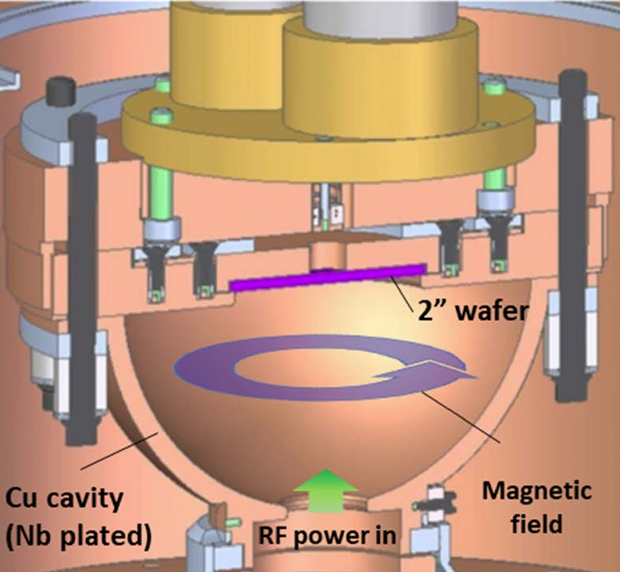
\includegraphics[width=0.7\linewidth]{images/Mushroom/MushroomCavity.png}
            \caption{SLAC mushroom cavity schematic, where the 2-inch wafer is the superconducting sample of interest, and the Cu cavity below is the host structure~\cite{sundahlDevelopmentCharacterizationNb3Sn2021}.}
            \label{fig:MushroomCavity}
        \end{figure}

    Mushroom-cavity testing separates material properties from full-cavity complications such as seam resistance, geometric errors, or coupling losses. Testing multiple small samples from one batch uses less material and time than coating full cavities. However, mushroom measurements have significant limitations: they cannot perform magnetic-field dependence measurements because they are too large to fit inside magnets, and the Nb host cavities would also break down in high magnetic fields. This means mushroom cavity tests cannot assess actual axion detector conditions near 9~T. 
    
    The Cu-Sn first approach discussed in Sec.~\ref{sec:nb3snresults} had its origin in depositing Nb on bronze substrates~\cite{withanageRapidNbSn2021}. An opportunity to measure these films in RF became available. Although it took longer than expected due to the pandemic and other delays, this work was completed because the results are directly relevant to the coatings being developed and the questions being investigated in this dissertation. Mushroom cavity experiments were never able to explore everything required, and coating the entire cavity (option~2) was always envisioned.



    
    Two-inch bronze substrate Nb$_3$Sn samples were sent to SLAC for $Q$ measurements in a mushroom cavity. These samples were made with the same recipe found in~\cite{withanageRapidNbSn2021}, which is the basis for the Cu-Sn first approach in this dissertation, i.e., the hot-bronze and the hot-bronze + post-reaction method (seen in Fig.~\ref{fig:2inchBronzeSub}). The critical temperature curves of the bronze coupon samples from \citeauthor{withanageRapidNbSn2021}~\cite{withanageRapidNbSn2021}, are shown in Fig.~\ref{fig:WenuraBronzeTc}. These samples had a superconducting transition around $14-15$~K. The quality factor results from the SLAC mushroom cavity are shown in Fig.~\ref{fig:MushroomQvsT}. The experiment resulted in a value of $Q=1.2\times10^6$ and $Q=5.5\times10^5$ for the hot-bronze and the hot-bronze + post-reacted samples, respectively. This mushroom cavity result was measured using a Cu host cavity, which increased the error. SLAC plans to repeat these measurements with a Nb mushroom cavity, which will reduce the error in high-$Q$ films. 

        \begin{figure}[htb]
            \centering
            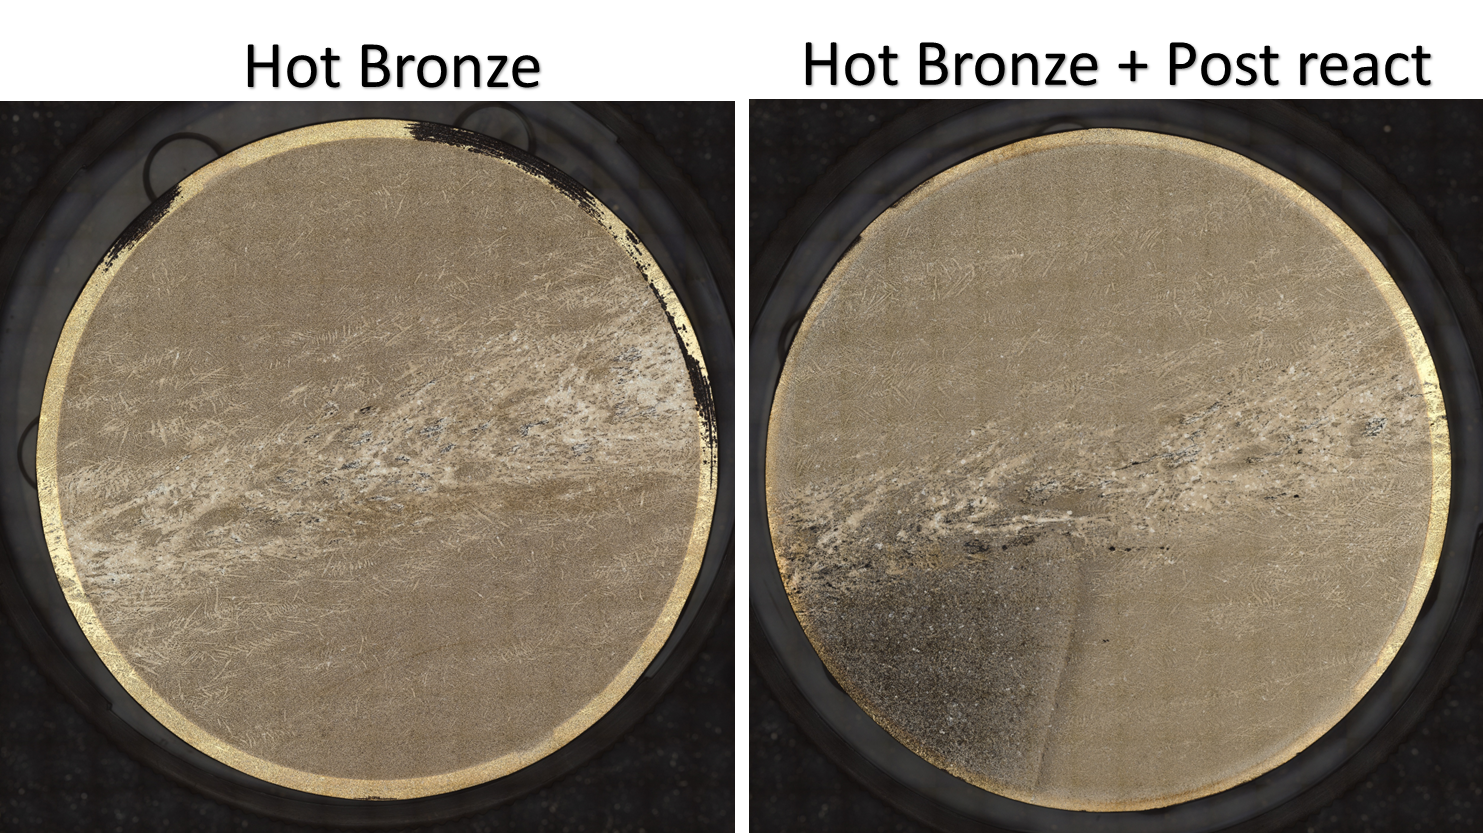
\includegraphics[width=0.9\linewidth]{images/Mushroom/2inchBronzeSub.png}
            \caption[The 2-inch bronze substrate disks, after Nb deposition and reaction, showing both the hot-bronze reaction, and the hot-bronze + a post-reaction.]{The 2-inch bronze substrate disks, after Nb deposition and reaction, showing both the hot-bronze reaction, and the hot-bronze + a post-reaction. The texture visible in the coatings is indicative of the underlying texture of the bronze substrates. These samples underwent the same heat-treatment as in bronze substrate samples found in \citeauthor{withanageRapidNbSn2021}~\cite{withanageRapidNbSn2021}.}
            \label{fig:2inchBronzeSub}
        \end{figure}

        
    
        \begin{figure}[htb]
            \centering
            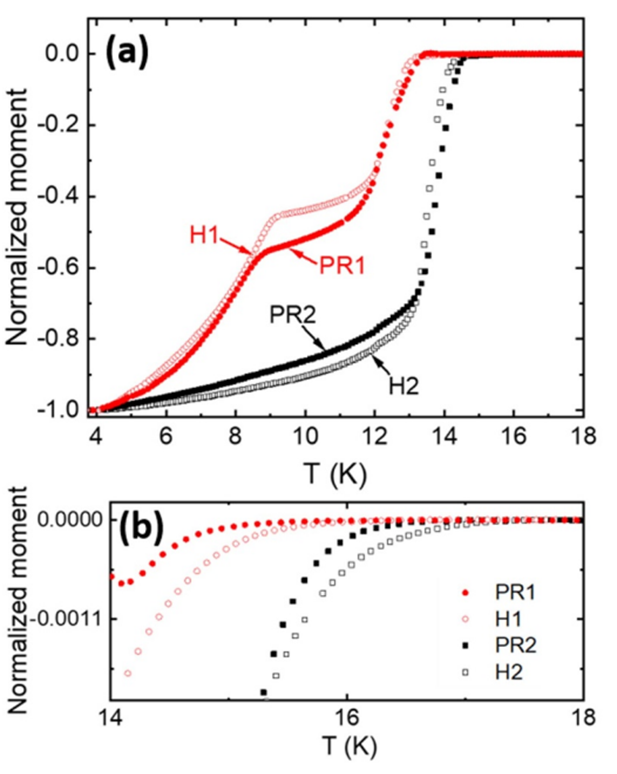
\includegraphics[width=0.5\linewidth]{images/Mushroom/WenuraBronzeTc.png}
            \caption{Samples marked with H2 and PR2 are coupon samples that underwent the same recipe as the 2-inch disk samples from the mushroom cavity measurement: hot-bronze, and hot-bronze + post-reaction, respectively~\cite{withanageRapidNbSn2021}.}
            \label{fig:WenuraBronzeTc}
        \end{figure}
        
    
    The hot-bronze + post-reacted sample has a darker region in the lower left, different from the rest of the sample (Fig.~\ref{fig:2inchBronzeSub}). This may be due to post-reaction effects that cause significant grain growth in the underlying bronze substrate. This can explain the drop in $Q$ for the post-reacted sample, even though this sample should have higher and more uniform Sn content than the hot-bronze sample based on $T_c$ curves (Fig.~\ref{fig:WenuraBronzeTc}). The patterning at the center of both samples is an artifact of rolling during the preparation of the bronze substrates. While mushroom cavity measurements provided initial $Q$ validation, $Q$ vs $B$ measurements were needed for accurate axion-detection relevant results. This led to the investigation and development of RF testing infrastructure in-house, to test $Q$ vs $B$.


        \begin{figure}[H]
            \centering
            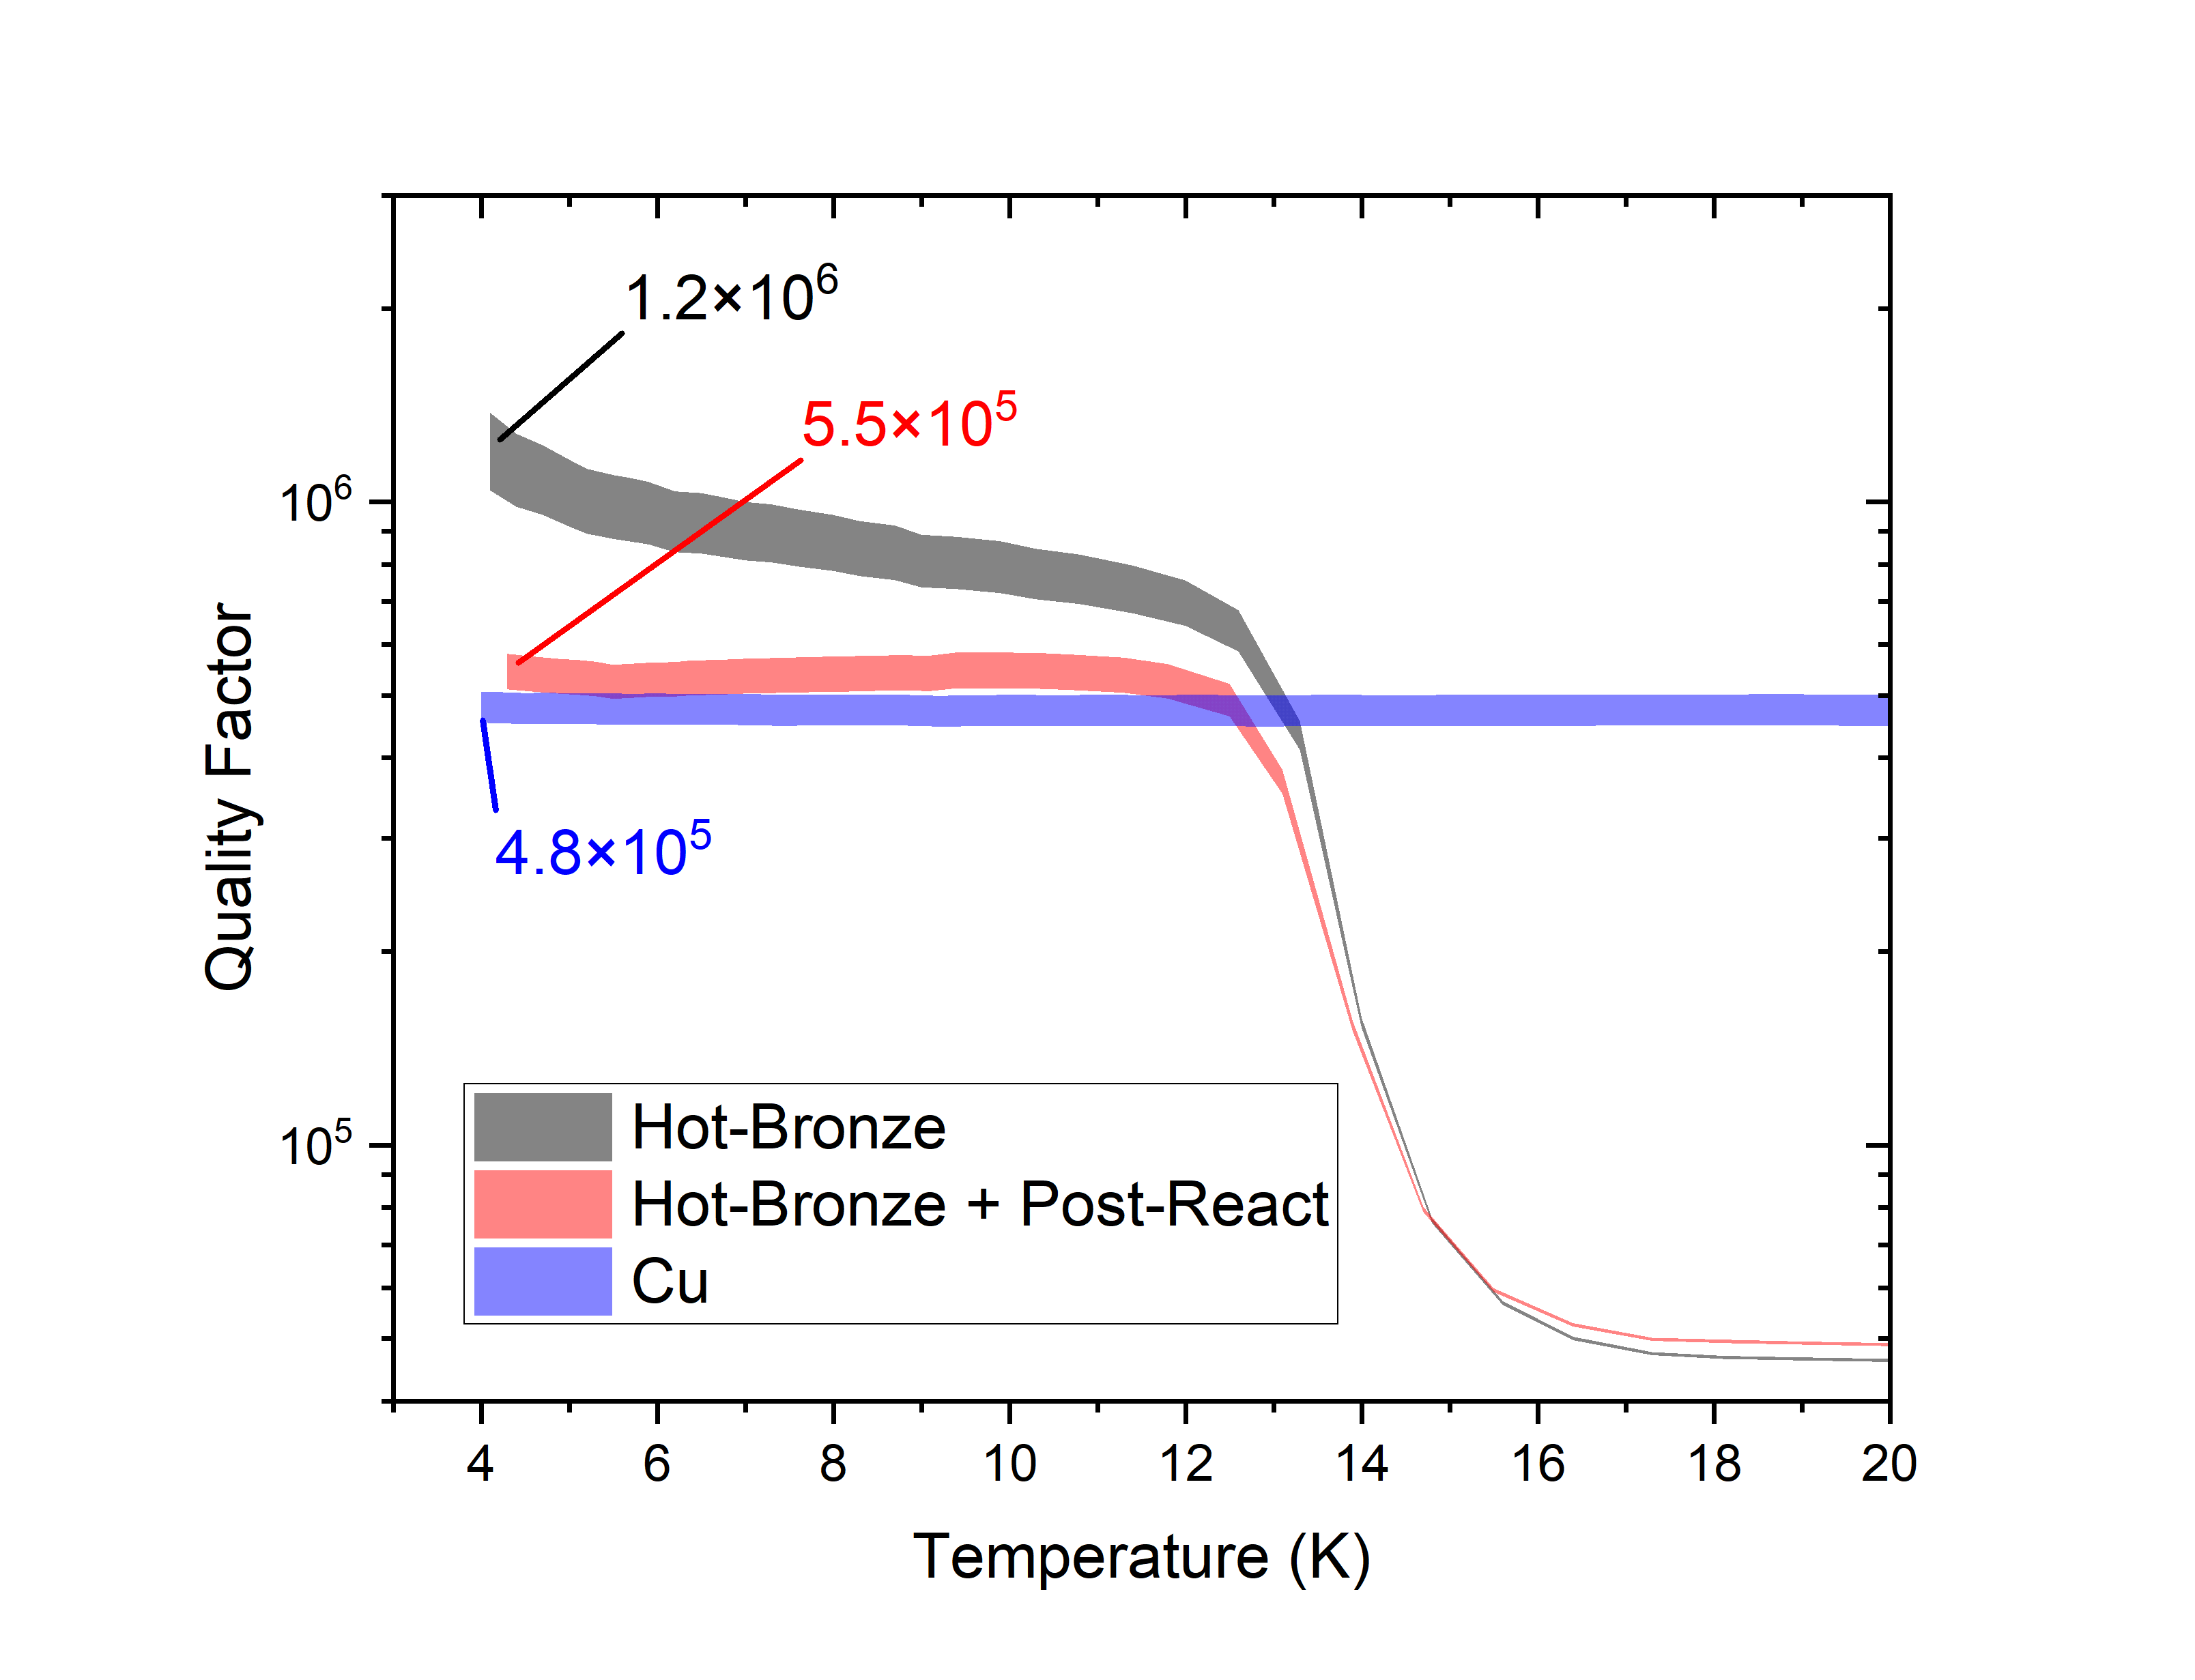
\includegraphics[width=0.7\linewidth]{images/Mushroom/QvsTMushroomCavityNew.png}
            \caption[Quality factor as a function of temperature for 2-inch bronze disk samples measured using the mushroom cavity at SLAC.]{Quality factor as a function of temperature for 2-inch bronze disk samples measured using the mushroom cavity at SLAC. The hot-bronze sample (deposited at elevated temperature) achieved $Q_0 = 1.2\times10^6$, while the hot-bronze sample with an additional post-deposition heat treatment achieved $Q_0 = 5.5\times10^5$. Both Nb$_3$Sn samples demonstrate higher quality factors than the bare Cu reference sample, confirming superconducting performance. Shaded regions indicate measurement uncertainty.}
            \label{fig:MushroomQvsT}
        \end{figure}
    \FloatBarrier


       
    
    \section{Superconducting RF Cavity}

    
    
    
    %Once we can measure the quality factor reliably, we can measure $Q$ while varying temperature and magnetic field. Both measurements use weak-coupling transmission with the cavity mounted in the PPMS, recording the resonant frequency and 3~dB bandwidth at each measurement point to extract Q via Eq.~\ref{eq:QVNA}. Both measurement types require allowing thermal equilibrium (5 minutes) after each parameter change before recording data to avoid transient effects. The measured Q$_L$ is converted to Q$_0$ using the coupling coefficients from reflection measurements (Eq.~\ref{eq:Q_0}).
        



    %We first need to design and model a cavity geometry that fits inside our magnet bore and our deposition system. Antenna ports must be added to input and output an RF signal into the interior of the cavity. We use CAD (FUSION) to design the model and input it into finite element simulations (COMSOL) to determine the electromagnetic resonance behavior of the geometry. After we are happy with the design and model, we machine the cavity. We then check where the cavity resonances lie in frequency space and find that the models have an error of +/- 1 MHz due to machining tolerances (error calculated from COMSOL).

    %Next radio-frequency (RF) cavity geometries are modeled and tested using COMSOL. The RF cavity walls are coated with an optimized recipe, and the cavity is placed in a PPMS, which allows for RF property testing while in an external magnetic field:

    A previous ADMX PhD student, Thomas Braine from the University of Washington, designed a cavity and probe that fits into small laboratory magnets (probe seen in Fig.~\ref{fig:ProbePPMSVNACavity})~\cite{Braine:2024nzi}. This dissertation partly adapts Braine's approach to allow measurements of $Q$ vs $B$ in the superconducting state using magnet systems available at the Applied Superconductivity Center. Braine's results show that a superconducting surface perpendicular to an external magnetic field incurs greater losses than when it is parallel to the field. This suggests a hybrid approach in which the top and bottom endcaps, which are perpendicular to the magnetic field, are normal-conducting Cu, and the walls parallel to the magnetic field are superconducting.

    The quality factor is the sum of all resonant surface losses in the cavity and depends on both surface resistance and geometry, as outlined in Chapter~\ref{sec:RFCharacterization}. Typical geometric factors for the first fundamental mode of 1.3~GHz Tesla cavities and 10~GHz cylindrical cavities are 270~$\Omega$~\cite{padamseeRFSuperconductivity2009} and 350~$\Omega$, respectively. The geometric factor for a given cavity and mode was calculated with a simulation. 

    
    \subsection{Axion Detector Cavity Methodology} \label{sec:RFCharacterization}


    To fully characterize the properties of a material for an axion detector application, quality factor measurements in external magnetic fields at low temperatures are required. This necessitates cooling the superconducting cavity to a low temperature, increasing the external magnetic field around the cavity, and measuring the quality factor. Cooling to cryogenic temperatures can be achieved with a helium cryostat or a cryocooler. A magnetic field can be created with a solenoid magnet. The magnet bore size (usable inner diameter of the magnet) presents the most significant constraint on the size and, therefore, frequency of the cavity. Measuring the quality factor requires stimulating the RF cavity surface of interest with AC power and measuring the ratio of reflected to absorbed power by the cavity walls. 
    
    It is important in axion detection to maximally couple the cavity's AC electric field and the external DC magnetic field, which depends on their dot product $\mathbf{E}_{\text{AC}} \cdot \mathbf{B}_0$. This requires a cavity mode where the electric field is parallel to the applied magnetic field. For a cylindrical cavity oriented vertically inside a solenoid magnet, the TM$_{010}$ mode produces an axial electric field aligned along the direction of the solenoid's axial magnetic field. The TM$_{010}$ is also the fundamental resonance, utilizing the full cavity volume without nodal planes that would reduce the effective interaction region. Therefore, when testing the cavity quality factor, a cylindrical cavity must be aligned with its axis along the magnetic field direction and the $Q$ of the TM$_{010}$ mode measured, thereby replicating the axion-detection electromagnetic field orientations.


    \subsubsection{Cavity Design}\label{sec:cavitydesign}

    The initial cavity design begins with an enclosed surface that provides the boundary conditions necessary for the formation of standing electromagnetic waves. A ``pillbox" cavity (cylinder) is commonly the starting geometry when describing a resonant cavity. This cylinder can be modeled using any computer-aided design (CAD) software and imported into a finite element simulation software. The cavity walls are modeled as boundary conditions with a specified conductivity, and an eigenfrequency study of this model will reveal the electromagnetic resonance behavior. This usually includes outputting the different oscillating modes with their respective geometric and quality factors. 

    Once the initial design and electromagnetic response of the cavity box is modeled, antenna ports (holes that lead from the exterior to the inner surface) must be added. This allows for input and output signals to be read from the cavity. Cavities are often made in two pieces due to machining and deposition constraints. It's difficult to machine a hollow volume with limited ports and deposit a superconductor on the inner surface. TESLA cavities used for accelerators have primarily been made in half-shells and electron-beam-welded together, but recent advances using hydroforming and other techniques have enabled the fabrication of full cavities from bulk, and Nb$_3$Sn recipes with cylindrical magnetrons or vapor are compatible with coating the inside of an enclosed cavity. However, it is much easier to inspect the surface when prototyping, so the design used here can be disassembled into two pieces, enabling machining, coating, and inspection with limited instrumentation. 

    \subsubsection{Physical Property Measurement System (PPMS)}

    The RF cavity testing stage presents particular experimental challenges. Measuring $Q$ at $9$~T and millikelvin temperatures requires careful consideration of magnet geometry. Magnet bore size limits the cavity dimensions and, therefore, the resonant frequency. For prototype designs using the widely available Physical Property Measurement System (PPMS) magnet, the magnet bore limits the cavity outer diameter to $<26$~mm. Accounting for wall thickness, this corresponds to resonant frequencies $\gtrsim 10$~GHz for cylindrical TM$_{010}$ cavities. This size constraint necessitates specialized probe design and cryogenic RF techniques. While larger-bore magnets ($40-100$~mm diameter) would permit lower-frequency cavities closer to axion-detection targets ($\sim4$~GHz), such systems require substantially more resources: higher capital costs, increased helium consumption, and limited availability. Constraining the design to PPMS-compatible dimensions enables rapid prototyping and accessibility across multiple laboratories.

    %\begin{figure}[tb]
    %    \centering
    %    
\includegraphics[width=0.9\linewidth]{images/AndreCavity/ProbePPMSVNACavity.png}
    %    \caption[Experimental apparatuses needed for Q measurement: probe, PPMS, cavity, VNA]{Experimental apparatuses needed for Q measurement: probe~\cite{Braine:2024nzi}, PPMS magnet, cavity, and VNA.}
    %    \label{fig:ProbePPMSVNACavity}
    %\end{figure}

    The PPMS (Quantum Design) provides high magnetic fields up to 9~T and cooling to 2~K. For quality factor testing, a specialized RF probe must connect the cavity inside the cold, high-field environment to a room-temperature vector network analyzer (VNA) for frequency response measurements. The probe and cavity must be constructed from non-magnetic materials (typically plastic (G10), copper, brass, or beryllium-copper), and all components must remain mechanically stable at cryogenic temperatures. The probe design, including RF feedthrough, is detailed in Ref.~\cite{Braine:2024nzi} and shown in Fig.~\ref{fig:ProbePPMSVNACavity}.

    Thermal load and thermal leakage to the environment must be considered, since the PPMS has limited cooling power. The PPMS is designed for small samples, so the cavity's large thermal mass increases helium consumption and cool-down times. However, if the probe sufficiently isolates the cavity from the external environment, the PPMS should be able to cool down the cavity to a stable 2~K using pot-fill mode. A Cernox temperature sensor is attached to the top of the cavity to ensure that the bottom and top are at thermal equilibrium. A Cernox can be attached to a cable that runs to the top of the probe, allowing for temperature measurements at the top of the cavity. The Cernox must be calibrated before cavity measurement to correctly correlate voltage to temperature.


    \subsubsection{Quality Factor vs Temperature}
            
    The cavity is cooled to base temperature (2~K) in zero applied field, and $Q$ is measured at increasing temperature steps (typically 0.5-1 K increments) past $T_c$. At low temperatures, the residual resistance due to trapped flux and material defects determines $Q$. As temperature increases, thermally-activated quasiparticles contribute additional losses through BCS surface resistance $R_\text{BCS} \propto \exp(-\Delta/k_BT)$, causing $Q$ to decrease exponentially. The temperature at which $Q$ begins to drop rapidly indicates the onset of a significant thermal quasiparticle population and helps verify the film's superconducting transition temperature.
    
    \subsubsection{Quality Factor vs Magnetic Field}
    
    Field-dependent measurements characterize the cavity's tolerance to external magnetic fields, which are critical for axion-detection applications. The cavity is maintained at a constant low temperature (2~K) while the applied magnetic field is increased from 0 to 9~T in steps of $0.25-1$~T. Below the lower critical field H$_{c1}$, the superconductor completely expels the magnetic field from its interior (Meissner state) and $Q$ remains relatively constant. Above H$_{c1}$, magnetic flux penetrates as quantized vortices, and their motion under RF creates additional dissipation. The field dependence of $Q$ reveals the effectiveness of flux pinning, the Campbell resistance $R_C$. 

    
    \subsubsection{Dilution Fridge Millikelvin Measurements}
    
    Dilution refrigerators use a mixture of $^3$He and $^4$He isotopes to reach temperatures as low as 10-100 mK. At these temperatures, the BCS surface resistance $R_\text{BCS} \propto \exp(-\Delta/k_BT)$ becomes exponentially suppressed. Millikelvin measurements isolate the temperature, independent contributions of surface resistance from trapped magnetic flux, grain boundaries, surface oxides, and other material defects, revealing the residual resistance R$_{0}$.
    
    Dilution refrigerator measurements are challenging due to complex setups, amplifiers, low input power required to limit stage heating, longer cooldown times, and limited availability, particularly for systems with high-field magnet capability. Given these constraints, the magnetic-field dependence was assessed using the PPMS, and the dilution fridge separately assessed ultra-low-temperature performance. Combining PPMS field data with dilution fridge temperature data allows performance estimation in axion detector operating conditions (mK temperatures, 9~T fields).

        

    \subsection{Recipe Selection for Cavity Fabrication}\label{sec:recipe3}

    Recipe 3 (Nb-first geometry) was selected for cavity coating (see Sec.~\ref{sec:nbfirst}) based on microstructural uniformity. SEM cross-sections demonstrated excellent Nb$_3$Sn thickness uniformity (Fig.~\ref{fig:BronzeOnNb}) and a sharp Ta/Nb$_3$Sn interface resulting from sequential in-vacuum deposition. This route sacrificed chemical uniformity (broader transitions and a lower $T_c$ onset compared to the Cu-Sn first routes, Recipe 1 \& 2) in favor of microstructural uniformity. However, Recipe 3 was chosen because RF surface resistance depends critically on lateral uniformity across the cavity surface.
    
    \subsection{RF Cavity Design Constraints}
        
    \noindent The design of RF cavities within the constraints discussed above should satisfy six goals:
    \begin{enumerate}
        \item Build a cavity that facilitates an optimization process to increase $Q$ at a temperature of 2~K and an external magnetic field of 9~T.
        \item The cavity pieces must fit inside the low-profile evaporator and sputtering chamber, i.e., no more than 13~mm thick (Fig.~\ref{fig:ClearenceSputter}).
        \item When assembled, the cavity outer diameter must be less than 26~mm to fit inside the bore of the magnet. This constrains the cavity frequency to be above 10 GHz. Comparing cavity properties with the literature requires accounting for the frequency difference.
        \item Cavity surfaces must be flat planes to make best use of the line-of-sight deposition sources.
        \item The design should allow for hybrid designs that interchange superconducting and normal-conducting materials for the surfaces of the walls and the endcaps.
        \item The resonator must fit within the magnet's 55 mm homogeneous field region.
    \end{enumerate}

    Braine's design, the starting point for the cavity design, had a curved surface that was not tailored to the deposition systems at the Applied Superconductivity Center (ASC). Inspiration came from the Korean group's REBCO "orange wedge" cavity discussed in Sec.~\ref{sec:KoreanRebco} and Fig.~\ref{fig:AhnREBCO}. By changing Braine's upright cylinder shape to an upright polygon, it became possible to conceive of a cavity that could be fabricated using methods directly derived from the Nb$_3$Sn thin-film approaches developed in this dissertation. Furthermore, both research groups noted opportunities to use electromagnetic models to account for behavior at end caps and seams. Thus, the two approaches were merged in this work to create a compact footprint for testing in actual RF conditions using equipment available to ASC.

    

    %Another possibility, rather than using Cu endcaps, is designing the cavity so that the endcaps and walls have minimal perpendicular field components, as is the case in the cigar cavity~\cite{Posen:2022tbs}.

    \subsection{Rational for Hexagonal Prisms}\label{sec:Simulation}

    Finite element simulations including resistive seam interfaces (Fig.~\ref{fig:GapnoGapCylinderHexagon}) revealed a key advantage for hexagonal geometry. Without seams, the hexagon has ~9\% lower $Q$ than a cylinder due to geometry alone. However, introducing two resistive seams on the wall (simulating an interface in a two-piece cavity), reduces cylinder $Q$ by ~27\% but hexagon $Q$ by only ~1\%. The hexagonal geometry naturally concentrates current away from the corners (current is concentrated at the center of the faces). If the seams are located on the corners, dissipation is reduced. In contrast, the cylinder's axial symmetry maintains uniform current distribution along the wall, leading to more current losses at the seams.

    \begin{figure}[htb]
        \centering
        
\includegraphics[width=0.8\linewidth]{images/AndreCavity/GapnoGapCylinderHexagon.png}
        \caption[COMSOL simulation showing the change of frequency and quality factor for the cylinder (a, b) and hexagon (c, d) geometries.]{COMSOL simulation showing the change of frequency and quality factor for the cylinder (a, b) and hexagon (c, d) geometries. The color scale shows the surface current, with red indicating maximum and green indicating minimum. Input surface resistance is 5 \unit{\mohm} for the walls and 1 \unit{\ohm} for the gap. Comparing b and d, we note that using the hexagonal cavity reduces the surface resistance lost when a seam is at the edge of the hexagonal cavity.}
        \label{fig:GapnoGapCylinderHexagon}
    \end{figure}

    \subsection{RF Quality Factor Measurement Protocol}

    %ADD VNA SPEC
    
    All cavity quality factor measurements were performed using a Keysight PNA vector network analyzer (VNA) with a frequency range up to 20~GHz. The VNA output power was set to 10~dBm, with an IF bandwidth of 1~kHz and 200 sweep points. For quality factor extraction, the frequency range was swept over three times the full-width at half-maximum (FWHM) centered on the resonance frequency. 
    
    Cavities were coupled to the VNA using weak coupling via transmission ($S_{21}$) measurements. Weak coupling was verified by reflection measurements showing a dip of less than 1~dB, ensuring that the loaded quality factor $Q_L$ differed from the unloaded quality factor $Q_0$ by less than 10\%. All quality factors reported in this chapter are loaded values ($Q_L$); the intrinsic cavity quality factor $Q_0$ is approximately 10\% higher.
    
    Temperature-dependent measurements in the Physical Property Measurement System (PPMS) allowed 1-minute equilibration time after the PPMS temperature stabilized before recording data. Magnetic field-dependent measurements used the fastest available ramp rate in the PPMS, with 1-minute hold time at each field value. Measurements were performed in 0.5~T steps from 0 to 9~T with the cavity axis aligned parallel to the magnetic field direction.
            
    \subsection{8-Piece Hexagonal Cavity}

    \subsubsection{8-Piece Cu Cavity Fabrication}

    
    \begin{figure}[ht]
        \centering
        
\includegraphics[width=0.75\linewidth]{images/AndreCavity/1stcavity.png}
        \caption{a) Side view and b) cross section of the 8-piece Cu cavity (6 walls, 2 endcaps).}
        \label{fig:1stcavity}
    \end{figure}

    %Check cavity dimensions

    The hexagonal cavity consisted of six separate walls and two endcaps machined from annealed oxygen-free high-conductivity (OFHC) copper at the National High Magnetic Field Laboratory machine shop. The cavity measured 75~mm in height with a hexagonal cross-section; each flat face was 13~mm wide. Wall thickness tapered from approximately 2~mm at the center to $<$0.5~mm near the vertices.

    Individual pieces were mechanically polished using the same procedure as coupon samples: progressive carbide paper (400--1200 grit), diamond slurry (5--1~\unit{\um}), and vibratory colloidal silica (0.05~\unit{\um}). The cavity was assembled using 12 hand-tightened stainless steel 2-56 screws. Antenna coupling was achieved through two gold-plated SMA female connectors mounted on the top endcap.

    %solder attachment, 2-hole flange-mount stub terminal, 0.481~inch hole spacing, 0.050~inch diameter pin, gold-plated)
    
    This segmented geometry enabled polishing and deposition on flat surfaces, reducing the risk of coating non-uniformity. However, the design required a trade-off: thinner walls reduced interior volume (increasing frequency-dependent losses), while the minimal thickness near the vertices compromised mechanical stability under thermal stresses during cooldown, induced currents during magnet ramping, and assembly misalignment.


    %The thickness of the walls near the hexagon's long edge was less than 1 mm. When the cavity was squeezed, the measurement became inconsistent, suggesting that $Q$ was dominated by RF leakage. We believe this limited our quality factor to 60\% from the ideal $Q$. However, we decided to coat one of the hexagonal cavity walls with our down-selected Nb first recipe (Recipe 3, described in Section \ref{sec:recipe3}) to test $Q$ as a function of temperature and magnetic field.

    Nonetheless, the 8-piece Cu prototype allowed RF measurement, which encouraged coating one of the six walls with Nb$_3$Sn using the Nb-first approach described in Sec.~\ref{sec:nbfirst}. This process is depicted in Fig.~\ref{fig:8pieceRecipe}. 

    \begin{figure}[ht]
        \centering
        
\includegraphics[width=0.75\linewidth]{images/AndreCavity/8pieceRecipe.png}
        \caption{Cavity wall from the 8-piece design that went through a full downselected Nb-first recipe.}
        \label{fig:8pieceRecipe}
    \end{figure}
    \FloatBarrier
    
    Because of the mechanical stability limitations encountered, it was decided not to attempt an 8-piece cavity with either 6 superconducting walls and 2 Cu endcaps or all 8 pieces coated with superconductor. Future work that overcomes challenges associated with mechanical stiffness and alignment could further explore this design with increased wall thickness. Increasing the magnet bore size for RF measurements would facilitate adding volume for thicker cavity pieces.

    \subsubsection{8-Piece Cavity Coating}

    One cavity wall was coated with Nb$_3$Sn using Recipe 3 (Nb-first approach, Section~\ref{sec:nbfirst}). Due to the non-standard geometry, a custom sample holder was fabricated to hold the hexagonal wall piece at the top edge, where the wall would interface with the endcaps, leaving the interior surface exposed for coating. The wall underwent the standard Recipe 3 process: a 500~nm Ta diffusion barrier, a 500~nm Nb seed layer, and a 5~\unit{\um} Cu-33~at.\% Sn thermally evaporated in steps, followed by post-reaction at 715~$^\circ$C for 3 hours, and finally Cu-Sn removal via ammonium persulfate etching. Visual inspection after coating revealed some film delamination, particularly near the edges where the holder contacted the substrate and at regions with steep geometry relative to the deposition flux direction (Fig.~\ref{fig:8pieceDelamination}).\

    \begin{figure}[htb]
        \centering
        
\includegraphics[width=\linewidth]{images/AndreCavity/8pieceDelamination.png}
        \caption{Delamination near the edge after heat-treatment for 8-piece cavity wall before and after etching.}
        \label{fig:8pieceDelamination}
    \end{figure}

    
    \subsubsection{8-piece Cavity Results}

    The assembled bare Cu cavity with antenna couplers achieved $Q = 9{,}000$ at room temperature and $Q = 33{,}000$ ($R_s = 11$~\unit{m\ohm}) at 4~K (1st cavity in Fig.~\ref{fig:CuCavitiesRsvsT}). These values fall below our simulated expectations for high-purity Cu ($RRR > 300$) with no RF leakage, which predict $Q = 13{,}500$ at room temperature and $Q = 77{,}000$ ($R_s = 5$~\unit{m\ohm}) at 4~K (as seen in simulation Fig.~\ref{fig:GapnoGapCylinderHexagon}). Temperature dependence on surface resistance is given in Fig.~\ref{fig:CuCavitiesRsvsT} with a comparison to the ideal at low temperature.

    The measured quality factor vs. temperature shows a clear superconducting transition, yielding a higher quality factor than that of bare Cu. Comparing the normalized surface resistance curve of the cavity to the critical temperature curve from our coupon sample (Fig.~\ref{fig:RSandMoment8Piece}) with the same recipe, the curves are in reasonable agreement, showing a $T_c$ around 15~K. This confirms that transferring our recipe from a coupon sample to a larger-scale cavity wall creates quantitatively similar Nb$_3$Sn. 

    \begin{figure}[htb]
        \centering
        
\includegraphics[width=0.5\linewidth]{images/AndreCavity/RSandMoment8Piece.png}
        \caption[Comparison between normalized cavity measurement and coupon sample SQUID measurement.]{Comparison between normalized cavity measurement and coupon sample SQUID measurement. This confirms the cavity's sensitivity to the superconducting material.}
        \label{fig:RSandMoment8Piece}
    \end{figure}
    
    The surface resistance of the one superconducting wall was extracted by comparing the pure Cu cavity to the Cu cavity with one superconducting wall. This calculated surface resistance is overlaid with the pure Cu and single wall cavity in Fig.~\ref{fig:8pieceCavityRCorrected}. The surface resistance of individual surfaces is calculated using the math found in Appendix \ref{app:Qcorrection}. The superconducting transition is apparent at 15~K, and the cavity losses become dominated by the Cu walls at around 13~K. This leads to a calculated surface resistance of $R_s \sim \qty{8}{m\ohm}$ for the Nb$_3$Sn wall compared to $R_s \sim \qty{11}{m\ohm}$ for Cu. 
    
    %There is a significant error in this calculation due to the small participation factor from the one superconducting wall.

    \begin{figure}
        \centering
        
\includegraphics[width=0.9\linewidth]{images/AndreCavity/8pieceCavityRCorrected.png}
        \caption{Model of 8 piece cavity with one Nb$_3$Sn wall and the $R_s$ vs $T$ curve for bulk Cu, cavity with one superconducting wall, and isolated superconducting wall.}
        \label{fig:8pieceCavityRCorrected}
    \end{figure}

    The quality factor vs. magnetic field for this cavity, shown in Fig.~\ref{fig:8pieceQvsB} at 2~K, exhibits a linear dependence on magnetic field. The superconducting wall was parallel to the magnetic field, so from geometrical considerations, low resistance should have been achieved with this hybrid geometry. At 8~T the superconducting state is lost, which is much lower than the predicted $>H_{c2}=20$~T commonly found in wires. At very low field $B_0<1$~T, the superconductor was more resistive than Cu. 
    
    %Because the film was both fragile (500~nm) and had roughness on the scale of this thickness, we believe the vortex axis had perpendicular components to the external magnet field. This leads to large Lorentz forces on the vortices, even though the wall is nominally parallel to the external magnetic field. We believe this to be the dominant mechanism for poor surface resistance in a magnetic field.
    
    %Vortex oscillation also occurs on a length scale larger than 500~nm $\lambda_c \sim \qty{1}{\um}$, so the magnetic field can penetrate the substrate (from partial screening), leading to high dissipation. This is especially true if the thin-film substrate interface contains highly resistive oxides. 
    
    \begin{figure}[htb]
        \centering
        
\includegraphics[width=0.75\linewidth]{images/AndreCavity/8pieceQvsB.png}
        \caption[Quality factor vs Magnetic field for the single wall 8-Piece cavity.]{Quality factor vs Magnetic field for the single wall 8-Piece cavity. At 8 tesla, the superconducting wall becomes normal conducting.}
        \label{fig:8pieceQvsB}
    \end{figure}

    This experiment proved promising as the first prototype. This design allowed a direct comparison of results from DC measurements on coupon samples with those from RF measurements on the larger cavity walls, demonstrating a new capability for ASC. Another important outcome was the first indication that the RF properties of the Nb$_3$Sn thin films produced by the methods researched in this dissertation can indeed lead to improvement of the quality factor over Cu-only alternatives. However, the results from the cavity were unsatisfactory due to both RF leakage in the design and the substantial degradation of $Q$ with the magnetic field. The main limitation of this design was the large number of high-resistance Cu-to-Cu interfaces (18). 
    
    \subsection{2-Piece Hexagonal Cavity: DOE Office of Science Graduate Student Fellowship project}

    The encouraging RF results from the mushroom cavity and 8-piece hexagonal cavity experiments motivated the writing of a proposal for a Department of Energy Office of Science Graduate Student Research (SCGSR) fellowship. The proposal was partnered with Dr. Gianpaolo Carosi at Lawrence Livermore National Laboratory (LLNL) and the research team that previously worked with the ADMX experiment and mentored Dr. Braine's thesis. The LLNL facility has equipment that permits testing of RF cavities for axion detectors down to $< 100$~mK temperature and in magnetic fields up to 9~T, similar to the capabilities at the ASC. The goal of the fellowship was to augment this dissertation by extending measurement capabilities to the millikelvin range and leveraging expertise in cavity design.
    
    \subsubsection{2-Piece Cavity Design and Fabrication}    
    
    The SCGSR proposal considered reducing the number of cavity interfaces by constructing a hexagonal cavity out of 2 pieces of solid Cu. This geometry was almost identical to Braine's cavity, except that the inner surface was hexagonal rather than cylindrical. The hexagon shape was retained to (a) fit in the sputtering chamber, (b) replicate the inner shape of the 8-piece cavity, (c) facilitate reasonably easy surface preparation and inspection, and (d) make use of the electromagnetic models that were developed to understand the RF properties of the 8-piece cavity. The 2-piece cavity has much thicker walls than the 8-piece cavity, thereby reducing uncertainties associated with RF leakage caused by low stiffness and misaligned edges.

    The 2-piece cavity design trades the improvements discussed above for more difficult surface polishing and less certainty in thin-film deposition. Four cavities were ordered from Xometry and machined from bulk OFHC 101 Cu. Each cavity consisted of two hexagonal prism halves with a total height of 72~mm, a hexagonal flat face length of 12.25~mm, and a minimum wall thickness of 2~mm. 
    
    After receiving the cavities, the inner hexagonal surfaces were hand-polished. Due to the acute inner corners, standard polishing procedures were adapted by wrapping sandpaper around an eraser to reach tight curves. Each grit level (400--1200) was polished for approximately 1 minute per surface. Before pursuing more sophisticated methods such as electropolishing, it was decided that the 1200-grit hand polish was sufficient for initial testing. 
    
    The two cavity halves were assembled using four hand-tightened stainless steel 4-40 screws and three alignment pegs to ensure close positioning of the mating faces. Despite the alignment pegs, a small gap remained at the center of the seam, where paper could be slipped through, indicating imperfect mechanical contact. The cavity was then fitted with antenna couplers and tested for quality factor in the Physical Property Measurement System (PPMS).

    
    %The diameter could have been reduced to keep the design a cylinder or use a hexagon and cut off the outer diameter to allow for clearance in the sputtering machine (Fig.~\ref{fig:ClearenceSputter}). The hexagon had the added benefit of providing a more planar surface perpendicular to the deposition target. With the cylinder, the side walls are 90$^\circ$ from the target. The hexagon side walls (if cut at the polygon edge) are only $60^\circ$ from the target (Fig.~\ref{fig:Angle8piece}). This will allow for a more uniform coating along the long edge of the cavity, especially when using thermal evaporation (line-of-sight deposition).

   \begin{figure}[htb]
        \centering
        
\includegraphics[width=0.75\linewidth]{images/AndreCavity/ClearenceSputter.png}
        \caption{Sputtering chamber max clearance, for substrate thickness.}
        \label{fig:ClearenceSputter}
    \end{figure}
   
    %\begin{figure}[htb]
    %    \centering
    %    
\includegraphics[width=0.5\linewidth]{images/AndreCavity/Angle8piece.png}
    %    \caption[Hexagonal vs cylindrical cavity inner surface angles relative to deposition]{Hexagonal and cylindrical 2-piece cavity design showing the angle normal to the direction of incoming physical vapor deposition. Zero degrees corresponds to a flat sample, and 90 degrees is the maximum angle that can be coated with line-of-sight methods such as thermal evaporation.}
    %    \label{fig:Angle8piece}
    %\end{figure}

    \begin{figure}[htb]
        \centering
        
\includegraphics[width=0.75\linewidth]{images/AndreCavity/2piececavityCu.png}
        \caption{2-piece Cu cavity.}
        \label{fig:2piececavityCu}
    \end{figure}

    
    \begin{figure}[htb]
        \centering
        
\includegraphics[width=0.75\linewidth]{images/AndreCavity/2piececavityrecipe.png}
        \caption{Downselected Nb-first recipe coated on the 2-piece cavity design.}
        \label{fig:2piececavityrecipe}
    \end{figure}

    \subsubsection{2-piece Cavity Coating}

    All coating was performed at Florida State University using a modified version of Recipe 3 (Nb-first approach). The primary modification was the use of high-power impulse magnetron sputtering (HiPIMS) for the Ta diffusion barrier instead of standard DC magnetron sputtering. HiPIMS parameters used were 800~V peak voltage and a 50~\unit{\um} duty cycle, producing a Ta layer approximately 300~nm thick. The remainder of the recipe followed the standard Nb-first process: a Nb seed layer sputtered onto the substrate, with the substrate rotated and heated, followed by Cu-33~at.\% Sn thermal evaporation deposited in steps with 30-second holds between increments. The thermal evaporator lacked both rotation and substrate heating capabilities, raising concerns about the uniformity of the Cu-Sn film on the concave hexagonal surface. After Cu-Sn deposition, the cavity underwent post-reaction at 715~$^\circ$C for 3 hours in the sputtering chamber, followed by Cu-Sn removal via ammonium persulfate etching.

    
    %We followed a similar recipe to the 8-piece cavity, with one change: we used a high-temperature HiPIMS Ta deposition for the diffusion barrier, as recent studies have shown that this creates a highly crystalline Ta film. 
    

    
    Due to the cavity's concave geometry, the first non-flat substrate attempted in our fabrication process lacked a mask protecting the endcaps during deposition. A decision not to use a mask was made due to concerns about the added height and risk of contacting the heating element during sample transfer. Consequently, both the hexagonal walls and endcaps received Nb$_3$Sn coating.
    
    Before coating, the cavity was processed at Lawrence Livermore National Laboratory (LLNL) using the facility-standard stainless steel etching protocol, consisting of sequential treatments with soap, HCl, a dichromate solution, and an antioxidant. Following the initial RF measurements of the coated cavity at ASC, the cavity was annealed at 250~$^\circ$C for 6 hours in a positive-pressure argon tube furnace (evacuated to $4\times10^{-5}$ Torr before argon backfill, 0.2 liters per minute flow rate) to improve the Cu residual resistivity ratio. After substrate preparation and coating, the cavity was tested at ASC from 2~K to 20~K and then shipped to LLNL for dilution-refrigerator testing down to 50~mK. All RF measurements at LLNL follow a protocol established at ASC (see Sec.\ref{sec:RFCharacterization}).

    \subsubsection{2-piece Cavity Results}
    
    The first experiments with the 2-piece hexagonal Cu cavity were aimed at understanding the extent to which material grade and machining artifacts affected its resonant properties relative to those of the 8-piece hexagonal cavity prototype. The 2-piece cavity displayed $Q=12,000$ at room temperature and $Q=35,000$ at 4~K. This was an improvement to the previous design, with lower RF leakage (higher $Q$ at room temperature), but the Cu surface purity remained a concern (same $Q$ at low temperature).
    
    The etching process at LLNL increased $Q$ to $49,000$, and annealing at 250~$^\circ$C for 6 hours in a vacuum furnace further raised $Q$ to $55,000$. With the new etched and annealed Cu cavity achieving higher $Q$'s, the cavity's inner surface was fully coated with the downselected recipe 3 (see Sec.~\ref{sec:nbfirst}). We measured the cavity quality factor down to 2~K in the PPMS and to 50~mK in a $_3$He dilution refrigerator at Livermore (Fig.~\ref{fig:LLNLDilutionQtest}). The loaded quality factor measured from 50~mK to 300~mK was constant at $Q_L=77,000$ ($R_s=5~$\unit{m\ohm}) and at 2~K was $Q_L=59,000$ ($R_s=6~$\unit{m\ohm}) as seen in Fig.~\ref{fig:2pieceCavityResults}. As discussed in Section~\ref{sec:Qantenna}, weak coupling conditions ensure that the unloaded quality factor $Q_0$ is approximately 10\% higher than the reported loaded values, i.e., $Q_0 \approx 85{,}000$ at 50~mK and $Q_0 \approx 65{,}000$ at 2~K.

    \begin{figure}[htb]
        \centering
        
\includegraphics[width=0.7\linewidth]{images/AndreCavity/CuCavitiesRsvsT.png}
        \caption[Surface Resistance vs Temperature for the two Cu cavity designs, and a comparison between no polish, and electro-polished for the 2 piece cavity.]{Surface Resistance vs Temperature for the two Cu cavity designs, and a comparison between no polish, and electro-polished for the 2 piece cavity. The ideal 5~\unit{m\ohm} line is numerically calculated by simulating the cavity geometry and imputing the conductivity of the walls of high-purity (RRR=300) Cu at 11~GHz.}
        \label{fig:CuCavitiesRsvsT}
    \end{figure}

    \begin{figure}[htb]
        \centering
        
\includegraphics[width=0.9\linewidth]{images/AndreCavity/LLNLDilutionQtest.png}
        \caption{Dilution fridge setup for $Q$ measurements of the 2-piece cavity in mK temperatures.}
        \label{fig:LLNLDilutionQtest}
    \end{figure}

    \begin{figure}[htb]
        \centering
        
\includegraphics[width=0.9\linewidth]{images/AndreCavity/2pieceCavityResults.png}
        \caption{Model and $R_s$ vs T for the 2-piece Nb$_3$Sn cavity.}
        \label{fig:2pieceCavityResults}
    \end{figure}

    \subsubsection{Corrections to 2-Piece Cavity Quality Factor}

    Visual inspection revealed significant coating defects: the film on both endcaps peeled away during Cu-Sn etching (Fig.~\ref{fig:EdgeEffect2piece}), indicating that the line-of-sight deposition did not effectively coat surfaces perpendicular to the deposition flux. Additionally, the walls showed clear non-uniformities, including dark spots, scratches, and rough patches, which are artifacts of surface preparation and deposition on steeply inclined surfaces. 
    
    Thus, the measured $Q = 77{,}000$ includes losses from both the uncoated Cu endcaps (Nb$_3$Sn peeled away) and RF leakage at the seams. To estimate the performance of a fully coated Nb$_3$Sn cavity with no seam losses, two corrections were applied:
    
    \textbf{Correction 1: Accounting for Cu Endcaps.} Visual inspection confirmed that approximately one-third of the cavity surface remained uncoated Cu (both endcaps and nearby wall regions). For a hybrid cavity with geometric factor $G_\text{total} = 350~\Omega$, the measured quality factor reflects losses from both materials:
    
    \begin{equation}
    \frac{1}{Q_\text{measured}} = \frac{R_{s,\text{Cu}}}{G_\text{Cu}} + \frac{R_{s,\text{Nb$_3$Sn}}}{G_\text{Nb$_3$Sn}}
    \end{equation}
    
    \noindent where $G_\text{Cu} = 1050~\Omega$ (1/3 surface coverage) and $G_\text{Nb$_3$Sn} = 525~\Omega$ (2/3 coverage). Using the measured Cu cavity surface resistance $R_{s,\text{Cu}} = 6.36~\text{m}\Omega$ at 50~mK and solving for the Nb$_3$Sn contribution yields $R_{s,\text{Nb$_3$Sn}} = 3.64~\text{m}\Omega$. A fully coated Nb$_3$Sn cavity would therefore achieve:
    
    \begin{equation}
    Q_\text{Nb$_3$Sn,full} = \frac{G_\text{total}}{R_{s,\text{Nb$_3$Sn}}} = \frac{350~\Omega}{3.64~\text{m}\Omega} = 9.6 \times 10^4
    \end{equation}
    
    \textbf{Correction 2: Accounting for RF Leakage.} The measured Cu cavity showed RF leakage at seams, reducing $Q_\text{Cu,measured} = 55{,}000$ below the simulated ideal value $Q_\text{Cu,ideal} = 76{,}000$ for seamless geometry. Assuming the same fractional leakage affects the Nb$_3$Sn measurement, the correction factor is:
    
    \begin{equation}
    \alpha = \frac{Q_\text{Cu,ideal}}{Q_\text{Cu,measured}} = \frac{76{,}000}{55{,}000} = 1.38
    \end{equation}
    
    Applying this correction:
    
    \begin{equation}
    Q_\text{Nb$_3$Sn,corrected} = \alpha \times Q_\text{Nb$_3$Sn,full} = 1.38 \times (9.6 \times 10^4) = 1.3 \times 10^5
    \end{equation}
    
    \noindent at $B = 0$ and $T = 50$~mK. This corrected value represents the expected performance for an ideal fully coated Nb$_3$Sn cavity with no seam losses. It should be noted that all reported quality factors in this analysis are loaded values ($Q_L$); the intrinsic unloaded quality factor $Q_0$ would be approximately 10\% higher, giving $Q_{0,\text{corrected}} \approx 1.4 \times 10^5$ for the ideal Nb$_3$Sn cavity. The detailed correction procedure is provided in Appendix~\ref{app:Qcorrection}. This is solid evidence that pathways exist for Nb$_3$Sn cavities on Cu substrates to provide improved performance for future dark-matter searches.
    
    
    \begin{figure}[htb]
        \centering
        
\includegraphics[width=0.75\linewidth]{images/AndreCavity/EdgeEffect2piece.png}
        \caption{Coating defects at edge regions and endcaps of the two-piece cavity, showing film delamination and non-uniform coverage.}
        \label{fig:EdgeEffect2piece}
    \end{figure}